\documentclass[12pt,letter]{article}
\usepackage[pass]{geometry}
\usepackage{amssymb}

\usepackage{graphicx}
\usepackage{hyperref}
\newcommand*{\addheight}[2][.5ex]{%
  \raisebox{0pt}[\dimexpr\height+(#1)\relax]{#2}%
}

%%%%% ----------------------------------------

\usepackage{color}
\definecolor{gray97}{gray}{.97}
\definecolor{gray75}{gray}{.75}
\definecolor{gray45}{gray}{.45}

\usepackage{listings}
\lstset{ frame=Ltb,
framerule=0pt,
aboveskip=0.5cm,
framextopmargin=3pt,
framexbottommargin=3pt,
framexleftmargin=0.4cm,
framesep=0pt,
rulesep=.4pt,
backgroundcolor=\color{gray97},
rulesepcolor=\color{black},
%
stringstyle=\ttfamily,
showstringspaces = false,
basicstyle=\small\ttfamily,
commentstyle=\color{gray45},
keywordstyle=\bfseries,
%
numbers=left,
numbersep=15pt,
numberstyle=\tiny,
numberfirstline = false,
breaklines=true,
}

% minimizar fragmentado de listados
\lstnewenvironment{listing}[1][]
{\lstset{#1}\pagebreak[0]}{\pagebreak[0]}

\lstdefinestyle{consola}
{basicstyle=\scriptsize\bf\ttfamily,
backgroundcolor=\color{gray75},
}

\lstdefinestyle{C}
{language=bash,
}

\renewcommand{\figurename}{Figura}
%%%%% -----------------------------------------

\begin{document}
%\title{\centering{SMC aplicado a modelo de centro de masa de altura variable}}
\title{Reporte WRF}
\author{Joao Fabi\'an}
\date{ }
\maketitle 
\vspace{0.009cm}

\section*{Instalaci\'on}
La instalaci\'on del modelo WRF, del sistema de procesamiento WPS, y de los softwares de post-procesamiento, son realizados en distribuciones de Linux. Todas las secuencias y comandos mostrados en este reporte deben realizarse en el terminal de Linux, a no ser que se especifique lo contrario.\\

\noindent Se deben crear dos directorios en la \textit{carpeta de usuario} o \textit{home directory}. Un directorio ser\'a llamado \textit{Build\_WRF}, en este se montar\'an los archivos necesarios del modelo \textit{WRF}. El otro directorio ser\'a llamado \textit{TESTS}, y en este se montar\'an archivos que permitir\'an realizar pruebas para confirmar que el software adicional requerido funciona correctamente.

\subsection*{Software adicional requerido}
Es necesario instalar: \textit{gfortran}, \textit{csh}, \textit{m4} y  \textit{build-essential.} 
\begin{lstlisting}[language=bash]
$ sudo apt-get install gfortran csh m4 build-essential
\end{lstlisting}
					
\subsubsection*{Prueba del entorno del sistema}
Se deben tener instalados compiladores de \textit{Fortran} (gfortran), \textit{C++} (gpp) y \textit{C} (gcc), actualizados en sus versiones m\'as recientes.\\

\noindent Es necesario descargar los archivos que servir\'an para hacer las pruebas.
\begin{lstlisting}[language=bash]
$ cd ~/TESTS
$ wget http://www2.mmm.ucar.edu/wrf/OnLineTutorial/compile_tutorial/tar_files/Fortran_C_tests.tar
$ tar -xvf Fortran_C_tests.tar
\end{lstlisting}

\noindent Son siete pruebas que se encuentran disponibles. Estas se correr\'an una por una. 

\begin{enumerate}
\item Prueba para \textit{Fortran} de formato fijo:
\begin{lstlisting}[language=bash]
$ gfortran TEST_1_fortran_only_fixed.f
$ ./a.out
\end{lstlisting}

En caso de que la prueba sea exitosa, en el terminal se mostrar\'a:
\begin{lstlisting}[language=bash]
SUCCESS test 1 fortran only fixed format
\end{lstlisting}

\item Prueba para \textit{Fortran} de formato libre:
\begin{lstlisting}[language=bash]
$ gfortran TEST_2_fortran_only_free.f90
$ ./a.out
\end{lstlisting}

En caso de que la prueba sea exitosa, en el terminal se mostrar\'a:
\begin{lstlisting}[language=bash]
SUCCESS test 2 fortran only free format
\end{lstlisting}

\item Prueba de \textit{C}:
\begin{lstlisting}[language=bash]
$ gcc TEST_3_c_only.c
$ ./a.out
\end{lstlisting}

En caso de que la prueba sea exitosa, en el terminal se mostrar\'a:
\begin{lstlisting}[language=bash]
SUCCESS test 3 C only
\end{lstlisting}

\item Prueba de \textit{Fortran} llamando a una funci\'on en \textit{C}:
\begin{lstlisting}[language=bash]
$ gcc -c -m64 TEST_4_fortran+c_c.c
$ gfortran -c -m64 TEST_4_fortran+c_f.f90
$ gfortran -m64 TEST_4_fortran+c_f.o TEST_4_fortran+c_c.o
$ ./a.out
\end{lstlisting}

En caso de que la prueba sea exitosa, en el terminal se mostrar\'a:
\begin{lstlisting}[language=bash]
C function called by Fortran
Values are xx = 2.00 and ii= 1
SUCCESS test 4 fortran calling c
\end{lstlisting}


\item Prueba de \textit{csh}:
\begin{lstlisting}[language=bash]
$ csh TEST_csh.csh
\end{lstlisting}

En caso de que la prueba sea exitosa, en el terminal se mostrar\'a:
\begin{lstlisting}[language=bash]
SUCCESS csh test
\end{lstlisting}

\item Prueba de \textit{Perl}:
\begin{lstlisting}[language=bash]
$ ./TEST_perl.pl
\end{lstlisting}

En caso de que la prueba sea exitosa, en el terminal se mostrar\'a:
\begin{lstlisting}[language=bash]
SUCCESS perl test
\end{lstlisting}

\item Prueba de \textit{sh}:
\begin{lstlisting}[language=bash]
$ ./TEST_sh.sh
\end{lstlisting}

En caso de que la prueba sea exitosa, en el terminal se mostrar\'a:
\begin{lstlisting}[language=bash]
SUCCESS sh test
\end{lstlisting}

\end{enumerate}

\subsection*{Construcci\'on de librer\'ias}

Se crea el directorio \textit{LIBRARIES}:

\begin{lstlisting}[language=bash]
$ mkdir ~/Build_WRF/LIBRARIES
\end{lstlisting}

\noindent Se descargan los archivos comprimidos de las librer\'ias: \textit{MPICH}, \textit{NetCDF}, \textit{JasPer}, \textit{libpng} y \textit{zlib}:
\begin{lstlisting}[language=bash]
$ cd ~/Build_WRF/LIBRARIES
$ wget http://www2.mmm.ucar.edu/wrf/OnLineTutorial/compile_tutorial/tar_files/mpich-3.0.4.tar.gz
$ wget http://www2.mmm.ucar.edu/wrf/OnLineTutorial/compile_tutorial/tar_files/netcdf-4.1.3.tar.gz
$ http://www2.mmm.ucar.edu/wrf/OnLineTutorial/compile_tutorial/tar_files/jasper-1.900.1.tar.gz
$ http://www2.mmm.ucar.edu/wrf/OnLineTutorial/compile_tutorial/tar_files/libpng-1.2.50.tar.gz
$ http://www2.mmm.ucar.edu/wrf/OnLineTutorial/compile_tutorial/tar_files/zlib-1.2.7.tar.gz
\end{lstlisting}

\subsubsection*{Configuraci\'on de NetCDF}
\noindent Se abre el archivo \textit{.bashrc} que se encuentra en el \textit{home directory}:
\begin{lstlisting}[language=bash]
$ sudo nano ~/.bashrc
\end{lstlisting}

\noindent As\'i, al final del archivo \textit{.bashrc} se deben agregar las l\'ineas:
\begin{lstlisting}[language=bash]
# WRF environment variables
export DIR=/home/lmc/Build_WRF/LIBRARIES
export CC=gcc
export CXX=g++
export FC=gfortran
export CFLAGS=-m64
export F77=gfortran
export FFLAGS=-m64
\end{lstlisting}

\noindent Se corre \textit{.bashrc} y se descomprime el archivo correspondiente a \textit{NetCDF}:

\begin{lstlisting}[language=bash]
$ source ~/.bashrc
$ cd ~/Build_WRF/LIBRARIES
$ tar -zxvf netcdf-4.1.3.tar.gz
\end{lstlisting}

\noindent Se corre el archivo de configuraci\'on de \textit{NetCDF}:
\begin{lstlisting}[language=bash]
$ cd ~/Build_WRF/LIBRARIES/netcdf-4.1.3
$ ./configure --prefix=$DIR/netcdf --disable-dap --disable-netcdf-4 --disable-shared
$ make
$ make install
\end{lstlisting}

\noindent Se debe modificar otra vez el archivo \textit{.bashrc}:
\begin{lstlisting}[language=bash]
$ sudo nano ~/.bashrc
\end{lstlisting}

\noindent Al final del archivo \textit{bashrc} se deben agregar las siguientes l\'ineas:
\begin{lstlisting}[language=bash]
export PATH=$DIR/netcdf/bin:$PATH
export NETCDF=$DIR/netcdf
\end{lstlisting}

\noindent Se corre \textit{.bashrc}:
\begin{lstlisting}[language=bash]
$ source ~/.bashrc
\end{lstlisting}

\subsubsection*{Configuraci\'on de MPICH}
Se descomprime el archivo correspondiente a \textit{MPICH}:
\begin{lstlisting}[language=bash]
$ cd ~/Build_WRF/LIBRARIES
$ tar -zxvf mpich-3.0.4.tar.gz
\end{lstlisting}

\noindent Se corre el archivo de configuraci\'on de MPICH:
\begin{lstlisting}[language=bash]
$ cd ~/Build_WRF/LIBRARIES/mpich-3.0.4
$ ./configure --prefix=$DIR/mpich
$ make
$ make install
\end{lstlisting}

\noindent Se abre el archivo \textit{.bashrc} que se encuentra en el \textit{home directory}:
\begin{lstlisting}[language=bash]
$ sudo nano ~/.bashrc
\end{lstlisting}

\noindent Al final del archivo \textit{.bashrc}, se agrega la l\'inea:
\begin{lstlisting}[language=bash]
export PATH=$DIR/mpich/bin:$PATH
\end{lstlisting}

\noindent Se corre \textit{.bashrc}:
\begin{lstlisting}[language=bash]
$ source ~/.bashrc
\end{lstlisting}

\subsubsection*{Configuraci\'on de zlib}
Se descomprime el archivo correspondiente a \textit{zlib}:

\begin{lstlisting}[language=bash]
$ cd ~/Build_WRF/LIBRARIES
$ tar -zxvf zlib-1.2.7.tar.gz 
\end{lstlisting}

\noindent Se abre el archivo \textit{.bashrc} que se encuentra en el \textit{home directory}:
\begin{lstlisting}[language=bash]
$ sudo nano ~/.bashrc
\end{lstlisting}

\noindent Al final del archivo \textit{.bashrc} se agregan las líneas:
\begin{lstlisting}[language=bash]
export LDFLAGS=-L$DIR/grib2/lib
export CPPFLAGS=-I$DIR/grib2/include
\end{lstlisting}

\noindent Se corre \textit{.bashrc}:
\begin{lstlisting}[language=bash]
$ source ~/.bashrc
\end{lstlisting}

\noindent Se corre el archivo de configuraci\'on de \textit{zlib}:
\begin{lstlisting}[language=bash]
$ cd ~/Build_WRF/LIBRARIES/zlib-1.2.7
$ ./configure --prefix=$DIR/grib2
$ make
$ make install
\end{lstlisting}

\subsubsection*{Configuraci\'on de libpng}

Se descomprime el archivo correspondiente a \textit{libpng}:
\begin{lstlisting}[language=bash]
$ cd ~/Build_WRF/libraries
$ tar -zxvf libpng-1.2.50.tar.gz
\end{lstlisting}

\noindent Se corre el archivo de configuraci\'on de \textit{libpng}:
\begin{lstlisting}[language=bash]
$ cd ~/Build_WRF/LIBRARIES/libpng-1.2.50
$ ./configure --prefix=$DIR/grib2
$ make
$ make install

\end{lstlisting}

\subsubsection*{Configuraci\'on de JasPer}
Se descomprime el archivo correspondiente a \textit{Jasper}

\begin{lstlisting}[language=bash]
$ cd ~/Build_WRF/LIBRARIES
$ tar -zxvf jasper-1.900.1.tar.gz
\end{lstlisting}

\noindent Se corre el archivo de configuraci\'on de \textit{JasPer}:
\begin{lstlisting}[language=bash]
$ cd ~/Build_WRF/LIBRARIES/jasper-1.900.1
$ ./configure --prefix=$DIR/grib2
$ make
$ make install
\end{lstlisting}

\subsubsection*{Prueba de compatibilidad de librer\'ias con WRF y WPS}
Se descargan los archivos de pruebas:
\begin{lstlisting}[language=bash]
$ cd ~/TESTS
$ wget http://www2.mmm.ucar.edu/wrf/OnLineTutorial/compile_tutorial/tar_files/Fortran_C_NETCDF_MPI_tests.tar
$ tar -xvf Fortran_C_NETCDF_MPI_tests.tar
\end{lstlisting}

\noindent Son dos pruebas, y se realizar\'an una por una:
\begin{enumerate}
\item Prueba de Fortran + C + NetCDF:
\begin{lstlisting}[language=bash]
$ cd ~/TESTS
$ cp ${NETCDF}/include/netcdf.inc .
$ gfortran -c 01_fortran+c+netcdf_f.f
$ gcc -c 01_fortran+c+netcdf_c.c
$ gfortran 01_fortran+c+netcdf_f.o 01_fortran+c+netcdf_c.o -L${NETCDF}/lib -lnetcdff -lnetcdf
$ ./a.out
\end{lstlisting}

En caso de que la prueba sea exitosa, el terminal mostrar\'a:
\begin{lstlisting}[language=bash]
C function called by Fortran
Values are xx = 2.00 and ii = 1
SUCCESS test 1 fortran + c + netcdf
\end{lstlisting}

\item Prueba de Fortran + C + NetCDF + MPI:
\begin{lstlisting}
$ cd ~/TESTS
$ cp ${NETCDF}/include/netcdf.inc .
$ mpif90 -c 02_fortran+c+netcdf+mpi_f.f
$ mpicc -c 02_fortran+c+netcdf+mpi_c.c
$ mpif90 02_fortran+c+netcdf+mpi_f.o 02_fortran+c+netcdf+mpi_c.o -L${NETCDF}/lib -lnetcdff -lnetcdf
$ mpirun ./a.out
\end{lstlisting}

En caso de que la prueba sea exitosa, el terminal mostrar\'a:
\begin{lstlisting}[language=bash]
C function called by Fortran
Values are xx = 2.00 and ii = 1
status = 		2
SUCCESS test 2 fortran + c + netcdf + mpi
\end{lstlisting}
\end{enumerate}

\subsection*{Construcci\'on de WRF V4}
Se descarga WRF:
\begin{lstlisting}[language=bash]
$ cd ~/Build_WRF
$ wget http://www2.mmm.ucar.edu/wrf/src/WRFV4.0.TAR.gz
$ tar -zxvf WRFV4.0.TAR.gz
\end{lstlisting}

\noindent Se corre el archivo de configuraci\'on de WRF:
\begin{lstlisting}[language=bash]
$ cd ~/Build_WRF/WRF
$ ./configure
$ 34
\end{lstlisting}
Se escoge la opci\'on \textbf{34} debido a que la computadora presenta varios n\'ucleos, y permite trabajar en paralelo, adem\'as, se trabajar\'a con \textit{gfortran/gcc}.\\

\noindent Una vez que la configuraci\'on se complete, debe haberse generado un archivo llamado \textit{configure.wrf} en el mismo directorio.\\

\noindent Puesto que la configuraci\'on est\'a completa, se pasa a compilar, seleccionando el caso de acuerdo al prop\'osito para el que ser\'a usado el modelo \textit{WRF}. En este caso, se compila \textit{WRF} para casos reales:

\begin{lstlisting}[language=bash]
$ cd ~/Build_WRF/WRF
$ ./compile em_real >& compile.log &
$ tail -f compile.log
\end{lstlisting}

\noindent Para corroborar que la compilaci\'on fue exitosa, se revisa el directorio \textit{WRF}:
\begin{lstlisting}[language=bash]
$ cd ~/Build_WRF/WRF
$ ls -las main/*.exe
\end{lstlisting}

\noindent La compilaci\'on se habr\'a completado correctamente si en el terminal se observan los ejecutables:

\begin{lstlisting}[language=bash]
main/ndown.exe
main/real.exe
main/tc.exe
main/wrf.exe
\end{lstlisting}


\subsection*{Construcci\'on de WPS V4}
El programa \textit{WPS} debe construirse debido a que se busca trabajar con casos reales.\\

\noindent Se descarga WPS:
\begin{lstlisting}[language=bash]
$ cd ~/Build_WRF
$ wget http://www2.mmm.ucar.edu/wrf/src/WPSV4.0.TAR.gz
$ tar -zxvf WPSV4.0.TAR.gz
$ cd WPS
$ ./clean
\end{lstlisting}

\noindent Se abre el archivo \textit{.bashrc}:
\begin{lstlisting}[language=bash]
$ sudo nano ~/.bashrc
\end{lstlisting}

\noindent Al final del archivo se agregan las l\'ineas:
\begin{lstlisting}[language=bash]
export JASPERLIB=$DIR/grib2/lib
export JASPERINC=$DIR/grib2/include
\end{lstlisting}

\noindent Se corre \textit{.bashrc}:
\begin{lstlisting}[language=bash]
$ source ~/.bashrc
\end{lstlisting}

\noindent Se corre el archivo de configuraci\'on de \textit{WPS}:
\begin{lstlisting}[language=bash]
$ cd ~/Build_WRF/WPS
$ ./configure
$ 1
\end{lstlisting}

\noindent Se selecciona la opci\'on \textbf{1} debido a las caracter\'isticas de la computadora, adem\'as de estar usando \textit{gfortran}. Si la configuraci\'on se completa correctamente, debe aparecer un mensaje en el terminal que terminar\'a con:

\begin{lstlisting}
This installation NetCDF is 64-bit
C compiler is 64-bit
Fortran compiler is 64-bit
\end{lstlisting}

\noindent El sistema \textit{WPS} debe direccionarse hacia las librer\'ias \textit{I/O} de \textit{WRF}, donde se encuentran los ejecutables \textit{metgrid.exe} y \textit{geogrid.exe}:

\begin{lstlisting}[language=bash]
$ cd ~/Build_WRS/WPS
$ sudo nano configure.wps
\end{lstlisting}
En el archivo, especificar la ruta hacia el directorio WRF:
\begin{lstlisting}[language=bash]
   WRF_DIR         =       ../WRF
\end{lstlisting}

\noindent Se compila \textit{WPS}:
\begin{lstlisting}[language=bash]
$ cd ~/Build_WRS/WPS
$ ./compile >& compile.log&
$ tail -f compile.log
\end{lstlisting}

\noindent Para corroborar que la compilaci\'on fue exitosa, revisar el directorio \textit{WPS}:
\begin{lstlisting}[language=bash]
$ cd ~/Build_WRS/WPS
$ ls -las *.exe
\end{lstlisting}

\noindent La compilaci\'on ser\'a correcta si en el terminal se muestran los ejecutables:
\begin{lstlisting}[language=bash]
geogrid.exe
metgrid.exe
ungrib.exe
\end{lstlisting}

\noindent Para inicializar casos reales, se deben crear la locaci\'on f\'isica del dominio en el goblo, y la informaci\'on est\'atica para tal locaci\'on. Esta informaci\'on debe ser descargada:

\begin{lstlisting}[language=bash]
$ cd ~/Build_WRF
$ wget http://www2.mmm.ucar.edu/wrf/src/wps_files/geog_10m.tar.gz
$ tar -zxvf geog_10m.tar.gz
$ mv geog WPS_GEOG
\end{lstlisting}

\noindent Se abre el archivo \textit{namelist.WPS}:
\begin{lstlisting}[language=bash]
$ cd ~/Build_WRF/WPS
$ nano namelist.wps
\end{lstlisting}

\noindent Se modifica el directorio correcto en el archivo \textit{namelist.wps}:
\begin{lstlisting}[language=bash]
geog_data_path= 	'/home/lmc/Build_WRF/WPS_GEOG/'
\end{lstlisting}
\subsection*{Post - Procesamiento}
Para poder leer los archivos generados por \textit{WRF} usando el core \textit{ARW}, se usa el programa \textit{ARWPost}, adem\'as, se usa \textit{GrADS} para poder hacer un plot de los resultados obtenidos.\\

\noindent Descargar ARWPost:
\begin{lstlisting}[language=bash]
$ cd ~/Build_WRF
$ wget http://www2.mmm.ucar.edu/wrf/src/ARWpost_V3.tar.gz
$ tar -zxvf ARWpost_V3.tar.gz
\end{lstlisting}

\noindent Asumiento que ya se configur\'o NetCDF, se configura ARWpost:
\begin{lstlisting}[language=bash]
$ cd ~/Build_WRF/ARWpost
$ ./configure
$ 3
$ cd src
\end{lstlisting}

\noindent Se abre el archivo \textit{Makefile}:
\begin{lstlisting}
$ cd ~/Build_WRF/ARWpost
$ sudo nano Makefile
\end{lstlisting}

\noindent En el archivo \textit{Makefile} se modifica la l\'inea correspondiente a \textit{ARWpost.exe}:
\begin{lstlisting}[language=bash]
ARWpost.exe: $(OBJS)
		$(FC) $(FFLAGS) $(LDFLAGS) -o $@ $(OBJS)  \
				-L$(NETCDF)/lib -lnetcdf -lnetcdff -I$(NETCDF)/include -lnetcdf
\end{lstlisting}

\noindent Adem\'as, se abre el archivo \textit{configure.arwp}:
\begin{lstlisting}[language=bash]
$ cd ~/Build_WRF/ARWpost
$ sudo nano configure.arwp
\end{lstlisting}

\noindent En el archivo \textit{configure.awps} se modifican las l\'ineas correspondientes a \textit{CFLAGS} y \textit{CPP}:
\begin{lstlisting}[language=bash]
CFLAGS		= 		-fPIC -m64
CPP		=		/lib/cpp -P -traditional
\end{lstlisting}

\noindent Se compila \textit{ARWpost}:
\begin{lstlisting}[language=bash]
$ cd ~/Build_WRF/ARWpost
$ ./compile
\end{lstlisting}

\noindent Se revisan los archivos generados, para comprobar si la compilaci\'on se realiz\'o de manera correcta:
\begin{lstlisting}[language=bash]
$ cd ~/Build_WRF/ARWpost
$ ls -ls *.exe
\end{lstlisting}

\noindent La compilaci\'on ser\'a correcta si el terminal muestra el ejecutable:
\begin{lstlisting}[language=bash]
ARWpost.exe
\end{lstlisting}

\noindent Para poder hacer un plot de los archivos que ser\'an generados a trav\'es de ARWpost, es necesario instalar el programa GrADS:

\begin{lstlisting}
$ sudo apt-get install grads
\end{lstlisting}
\section*{Pruebas}

\subsection*{Test 1}
\subsubsection*{Geogrid.exe}
En el procesamiento con WPS, se modifica el archivo \textit{namelist.wps}:
\begin{lstlisting}[language=bash]
$ cd ~/Build_WRF/WPS
$ sudo nano namelist.wps
\end{lstlisting}

\noindent As\'i, los par\'ametros en \textit{namelist.wps} son modificados de acuerdo a:

\begin{lstlisting}[language=bash]
wrf_core = 'ARW',
&share
 max_dom = 1,
 start_date = '2011-09-05_12:00:00','2006-08-16_12:00:00',
 end_date   = '2011-09-10_12:00:00','2006-08-16_12:00:00',
 interval_seconds = 10800
/

&geogrid
 parent_id         =   1,   1,
 parent_grid_ratio =   1,   3,
 i_parent_start    =   1,  31,
 j_parent_start    =   1,  17,
 e_we              =  15, 112,
 e_sn              =  15,  97,
 geog_data_res     = '2m','2m',
 dx = 3333.33,
 dy = 3333.33,
 map_proj = 'lambert',
 ref_lat   =  45.68,
 ref_lon   = -111.06,
 truelat1  =  30.0,
 truelat2  =  60.0,
 stand_lon = -111.06,
 geog_data_path = '/home/marv/Build_WRF/WPS_GEOG/'
/

&ungrib
 out_format = 'WPS',
 prefix = 'FILE',
/

&metgrid
 fg_name = 'FILE'
 io_form_metgrid = 2,
/

\end{lstlisting}
\noindent Se genera el ejecutable \textit{geogrid.exe}:
\begin{lstlisting}
$ cd ~/Build_WRF/WPS
$ ./geogrid.exe
\end{lstlisting}

\noindent El terminal indicar\'a el mensaje de confirmaci\'on siguiente:
\begin{lstlisting}
!!!!!!!!!!!!!!!!!!!!!!!!!!!!!!!!!!!!!!!!!!!!!!
!   Successful completion of geogrid.        !
!!!!!!!!!!!!!!!!!!!!!!!!!!!!!!!!!!!!!!!!!!!!!!
\end{lstlisting}

\subsubsection*{ungrib.exe}
El dataset usado es el \textbf{ds609.2}. Se realiza la descarga de este:
\begin{lstlisting}[language=bash]
$ mkdir ~/Build_WRF/data
$ mkdir ~/Build_WRF/data/AWIP_datasets
$ mkdir ~/Build_WRF/data/AWIP_datasets/ds609.2
$ cd ~/Build_WRF/data/AWIP_datasets/ds609.2
$ wget https://rda.ucar.edu/data/ds609.2/SFanal/2011/G43091.SFanal.201109
$ wget https://rda.ucar.edu/data/ds609.2/3Danal/2011/G43084.3Danal.201109.16-30
$ wget https://rda.ucar.edu/data/ds609.2/3Danal/2011/G43083.3Danal.201109.01-15
$ mv G43091.SFanal.201109 G43091.SFanal.201109.tar
$ mv G43084.3Danal.201109.16-30 G43084.3Danal.201109.16-30.tar
$ mv G43083.3Danal.201109.01-15 G43083.3Danal.201109.01-15.tar
$ tar -zxvf G43091.SFanal.201109.tar
$ tar -zxvf G43084.3Danal.201109.16-30.tar
$ tar -zxvf G43083.3Danal.201109.01-15.tar
\end{lstlisting}

\noindent Se genera el ejecutable \textit{ungrib.exe}:
\begin{lstlisting}
$ cd ~/Build_WRF/WPS
$ ln -sf ungrib/Variable_Tables/Vtable.AWIP Vtable
$ ./link_grib.csh ~/Build_WRF/AWIP_datasets/ds609.2/201109
$ ./ungrib.exe >& ungrib.log

\end{lstlisting}

\subsubsection*{metgrid.exe}
Se corre el ejecutable \textit{metgrid.exe}:

\begin{lstlisting}
$ cd ~/Build_WRF/WPS
$ ./metgrid.exe
\end{lstlisting}

\noindent El terminal indicar\'a el mensaje de confirmaci\'on siguiente:
\begin{lstlisting}
!!!!!!!!!!!!!!!!!!!!!!!!!!!!!!!!!!!!!!!!!!!!!!
!   Successful completion of metgrid.        !
!!!!!!!!!!!!!!!!!!!!!!!!!!!!!!!!!!!!!!!!!!!!!!
\end{lstlisting}

\subsubsection*{real.exe y wrf.exe}
Se entra al directorio \textit{test}:
\begin{lstlisting}[language=bash]
$ cd ~/Build_WRF/WRF/test/em_real
$ ln -sf ~/Build_WRF/WPS/met_em.d01.* .
$ sudo nano namelist.input
\end{lstlisting}

\noindent Los par\'ametros dentro del archivo \textit{namelist.input} se modifica de la forma:
\begin{lstlisting}[language=bash]
 &time_control
 run_days                            = 3,
 run_hours                           = 0,
 run_minutes                         = 0,
 run_seconds                         = 0,
 start_year                          = 2011, 2000, 2000,
 start_month                         = 09,   01,   01,
 start_day                           = 06,   24,   24,
 start_hour                          = 12,   12,   12,
 start_minute			     = 00,   00,   00,
 start_second                        = 00,   00,   00,
 end_year                            = 2011, 2000, 2000,
 end_month                           = 09,   01,   01,
 end_day                             = 09,   25,   25,
 end_hour                            = 12,   12,   12,
 end_minute                          = 00,   00,   00,
 end_second                          = 00,   00,   00,
 interval_seconds                    = 10800,
 input_from_file                     = .true.,.true.,.true.,
 history_interval                    = 180,  60,   60,
 frames_per_outfile                  = 1000, 1000, 1000,
 restart                             = .false.,
 restart_interval                    = 21600,
 io_form_history                     = 2,
 io_form_restart                     = 2,
 io_form_input                       = 2,
 io_form_boundary                    = 2,
 debug_level                         = 0,
 /

 &domains
 time_step                           = 30,
 time_step_fract_num                 = 0,
 time_step_fract_den                 = 1,
 max_dom                             = 1,
 s_we			             = 1,
 e_we                                = 15,    112,   94,
 s_sn                                = 1,
 e_sn                                = 15,    97,    91,
 s_vert                              = 1,
 e_vert                              = 60,    28,    28,
 p_top_requested                     = 5000,
 num_metgrid_levels                  = 27,
 num_metgrid_soil_levels             = 4,
 dx                                  = 3333.33, 10000,  3333.33,
 dy                                  = 3333.33, 10000,  3333.33,
 grid_id                             = 1,     2,     3,
 parent_id                           = 0,     1,     2,
 i_parent_start                      = 1,     31,    30,
 j_parent_start                      = 1,     17,    30,
 parent_grid_ratio                   = 1,     3,     3,
 parent_time_step_ratio              = 1,     3,     3,
 feedback                            = 1,
 smooth_option                       = 0,
 sfcp_to_sfcp = .true.
 /

 &physics
 physics_suite                       = 'CONUS'
 mp_physics                          = -1,    -1,    -1,
 cu_physics                          = -1,    -1,     0,
 ra_lw_physics                       = -1,    -1,    -1,
 ra_sw_physics                       = -1,    -1,    -1,
 bl_pbl_physics                      = -1,    -1,    -1,
 sf_sfclay_physics                   = -1,    -1,    -1,
 sf_surface_physics                  = -1,    -1,    -1,
 radt                                = 30,    30,    30,
 bldt                                = 0,     0,     0,
 cudt                                = 5,     5,     5,
 icloud                              = 1,
 num_land_cat                        = 21,
 sf_urban_physics                    = 0,     0,     0,
 /

 &fdda
 /

 &dynamics
 hybrid_opt                  = 2, 
 w_damping                   = 0,
 diff_opt                    = 1,      1,     1,
 km_opt                      = 4,      4,     4,
 diff_6th_opt                = 0,      0,     0,
 diff_6th_factor             = 0.12,   0.12,  0.12,
 base_temp                   = 290.
 damp_opt                    = 3,
 zdamp                       = 5000.,  5000.,  5000.,
 dampcoef                    = 0.2,    0.2,    0.2
 khdif                       = 0,      0,      0,
 kvdif                       = 0,      0,      0,
 non_hydrostatic             = .true., .true., .true.,
 moist_adv_opt               = 1,      1,      1,     
 scalar_adv_opt              = 1,      1,      1,     
 gwd_opt                     = 1,
 /

 &bdy_control
 spec_bdy_width                      = 5,
 specified                           = .true.
 /

 &grib2
 /

 &namelist_quilt
 nio_tasks_per_group = 0,
 nio_groups = 1,
 /
\end{lstlisting}

\noindent Para obtener los ejecutables \textit{real.exe} y \textit{wrf.exe}:
\begin{lstlisting}[language=bash]
$ ./real.exe
$ ./wrf.exe >& wrfoutput.log
\end{lstlisting}
Se generan archivos de salida correspondientes al procesamiento realizado haciendo uso de \textit{WRF}.

\subsubsection*{ARWpost}
Se ingresa al directorio \textit{ARWpost} y se modifica el archivo \textit{namelist.ARWpost}:
\begin{lstlisting}
$ cd ~/Build_WRF/WRF/ARWpost
$ sudo nano namelist.ARWpost
\end{lstlisting}

\noindent El archivo debe modificarse de la siguiente forma:
\begin{lstlisting}[language=bash]
&datetime
 start_date = '2000-01-24_12:00:00',
 end_date   = '2000-01-25_00:00:00',
 interval_seconds = 10800,
 tacc = 0,
 debug_level = 0,
/

&io
 input_root_name = '~/Build_WRF/WRF/test/em_real/wrfout_d01'
 output_root_name = './test'
 plot = 'all_list'
 fields = 'height,pressure,tk,tc'
 mercator_defs = .true.
/
 split_output = .true.
 frames_per_outfile = 2


 plot = 'all'
 plot = 'list' 
 plot = 'all_list'
! Below is a list of all available diagnostics
 fields = 'height,geopt,theta,tc,tk,td,td2,rh,rh2,umet,vmet,pressure,u10m,v10m,wdir,wspd,wd10,ws10,slp,mcape,mcin,lcl,lfc,cape,cin,dbz,max_dbz,clfr'
 

&interp
 interp_method = 0,
 interp_levels = 1000.,950.,900.,850.,800.,750.,700.,650.,600.,550.,500.,450.,400.,350.,300.,250.,200.,150.,100.,
/
extrapolate = .true.

 interp_method = 0,     ! 0 is model levels, -1 is nice height levels, 1 is user specified pressure/height

 interp_levels =    1000.,950.,900.,850.,800.,750.,700.,650.,600.,550.,
 500.,450.,400.,350.,300.,250.,200.,150.,100.,
 interp_levels = 0.25, 0.50, 0.75, 1.00, 2.00, 3.00, 4.00, 5.00, 6.00, 7.00, 8.00, 9.00, 10.0, 11.0, 12.0, 13.0, 14.0, 15.0, 16.0, 17.0, 18.0, 19.0, 20.0,

\end{lstlisting}

\noindent Se corre \textit{ARWpost.exe} para generar un archivo con extensi\'on \textit{.ctl} en el directorio especificado en \textit{namelist.ARWpost}:
\begin{lstlisting}[language=bash]
$ cd ~/Build_WRF/WRF/ARWpost
$ ./ARWpost.exe
\end{lstlisting}

\noindent Se va al directorio donde se gener\'o el archivo \textit{.ctl} para generar un gr\'afico a partir de este:
\begin{lstlisting}[language=bash]
$ ~/Build_WRF/ARWpost
$ grads
$ open test.ctl
$ d t2
\end{lstlisting}

\noindent El gr\'afico obtenido a partir de la variable \textbf{t2}, se muestra en la Figura 1.
\begin{figure}
\caption{Variable t2.}
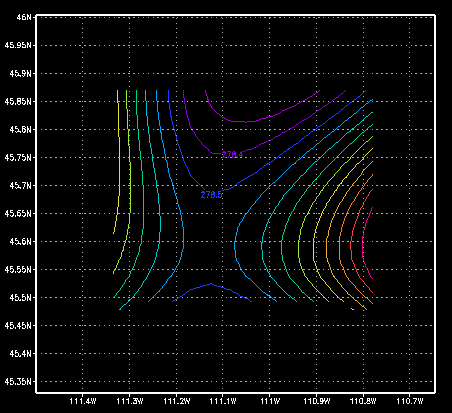
\includegraphics[scale=1]{grads_01.png}
\end{figure}

\noindent El gr\'afico obtenido a partir de la variable \textbf{tk}, se muestra en la Figura 2.

\begin{figure}
\caption{Variable tk.}
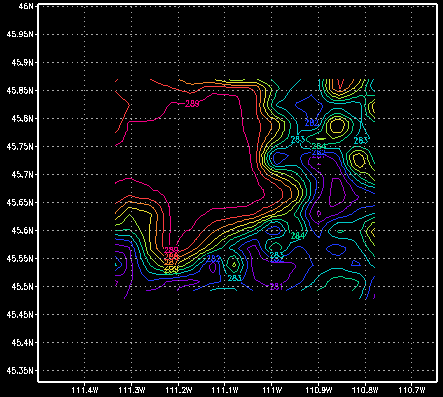
\includegraphics[scale=1]{grads_tk.png}
\end{figure}
\noindent El gr\'afico obtenido a partir de la variable \textbf{p} , se muestra en la Figura 3.

\begin{figure}
\caption{Variable p.}
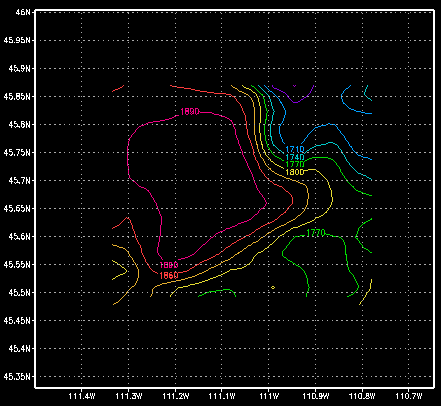
\includegraphics[scale=1]{grads_p.png}
\end{figure}
\noindent El gr\'afico obtenido a partir de la variable \textbf{v} , se muestra en la Figura 4.

\begin{figure}
\caption{Variable v.}
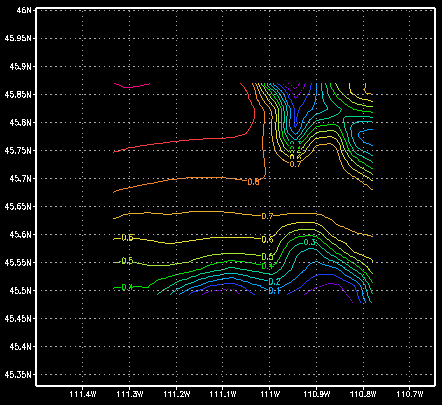
\includegraphics[scale=1]{grads_v.png}
\end{figure}
\clearpage
\section*{Observaciones}
\begin{itemize}
\item De acuerdo a los permisos del usuario que instale WRF, WPS y ARWpost; puede ser necesario tener permisos de "superusuario" para algunas tareas. Esta situaci\'on se encontr\'o principlamente al momento de correr ejecutables.

\item Al momento de ejecutar \textit{geogrid.exe}, dependiendo de la configuraci\'on del archivo \textit{namelist.wps}, pueden existir errores que indiquen la carencia de algunos datos. En este caso, los archivos pueden descargarse manualmente desde: \url{http://www2.mmm.ucar.edu/wrf/users/download/get_sources_wps_geog.html}

\item Al momento de ejecutar \textit{metgrid.exe}, pueden existir errores que indiquen inconsistencias con la configuraci\'on de \textit{geogrid.exe} y los par\'ametros en el archivo \textit{namelist.wps}. Se debe tener en cuenta que la generaci\'on de los ejecutables es secuencial, por lo tanto \textit{metgrid.exe} depende directamente de \textit{geogrid.exe}.

\item Algunos par\'ametros elegidos para compilar \textit{WRF} y \textit{WPS} dependen directamente de el equipo en el que se va a trabajar. El listado de opciones es mostrado directamente en el terminal, o puede ser visto en: \url{http://www2.mmm.ucar.edu/wrf/users/docs/user_guide_V3.9/users_guide_chap2.htm}
\end{itemize}



\end{document}